\documentclass[11pt,oneside,openany]{book}

\usepackage[
  paperwidth=16cm,
  paperheight=23cm,
  top=2.2cm,
  bottom=2.2cm,
  inner=2.4cm,
  outer=2cm
]{geometry}
\usepackage[T1]{fontenc}
\usepackage{tgpagella}
\usepackage{tgheros}
\usepackage[brazilian]{babel}
\usepackage{amsmath,amssymb}
\usepackage{graphicx}
\graphicspath{{recursos/}}
\usepackage{xcolor}
\usepackage{tikz}
\usepackage{csquotes}
\usepackage{etoolbox}
\usepackage[
  backend=biber,
  style=abnt
]{biblatex}
\addbibresource{referencias.bib}
\usepackage{hyperref}

\makeatletter
\patchcmd{\@makechapterhead}{\Huge}{\LARGE}{}{}
\patchcmd{\@makeschapterhead}{\Huge}{\LARGE}{}{}
\makeatother

\definecolor{booknavy}{HTML}{142A3B}
\definecolor{bookteal}{HTML}{2B7775}
\definecolor{bookgold}{HTML}{D8B56D}
\definecolor{bookpaper}{HTML}{F7F4EC}

\hypersetup{
  colorlinks=true,
  linkcolor=blue,
  citecolor=blue,
  urlcolor=blue,
  filecolor=blue,
  menucolor=blue,
  runcolor=blue,
  pdftitle={Sistemas Especialistas Integrados a Grandes Modelos de Inteligência Artificial},
  pdfsubject={Uma Coleção de Exemplos Práticos},
  pdfcreator={LaTeX}
}

\setlength{\parindent}{1.2em}
\setlength{\parskip}{0.25em}
\setcounter{tocdepth}{1}

\begin{document}
\pagestyle{plain}

\hypersetup{pageanchor=false}
\thispagestyle{empty}
\pagecolor{bookpaper}
\color{booknavy}
\begin{tikzpicture}[remember picture,overlay]
\begin{scope}[shift={(current page.south west)}]
\foreach \x in {-18,-14,-10,-6,-2,2,6,10,14,18,22} {
  \draw[bookteal,draw opacity=0.10,line width=0.45pt] (\x,0) -- ({\x+16},23);
  \draw[bookgold,draw opacity=0.09,line width=0.45pt] (\x,23) -- ({\x+16},0);
}
\begin{scope}[draw=bookteal,draw opacity=0.14,line width=0.5pt]
\draw (1.5,2) -- (4,3.5) -- (6.5,2.2);
\draw (1.5,4.7) -- (4,3.5) -- (6.5,4.8);
\draw (4,3.5) -- (4,5.8);
\draw (6.5,2.2) -- (9,3.5) -- (11.5,2.1);
\draw (6.5,4.8) -- (9,3.5) -- (11.5,4.9);
\draw (9,3.5) -- (9,5.9);
\draw (11.5,2.1) -- (14,3.4) -- (11.5,4.9);
\foreach \x/\y/\c in {1.5/2/bookgold,1.5/4.7/bookteal,4/3.5/bookteal,4/5.8/bookgold,6.5/2.2/bookgold,6.5/4.8/bookteal,9/3.5/bookgold,9/5.9/bookteal,11.5/2.1/bookteal,11.5/4.9/bookgold,14/3.4/bookteal} {\fill[\c,fill opacity=0.24] (\x,\y) circle (0.09);}
\draw (1.5,21) -- (4,19.5) -- (6.5,20.8);
\draw (1.5,18.3) -- (4,19.5) -- (6.5,18.2);
\draw (4,19.5) -- (4,17.2);
\draw (6.5,20.8) -- (9,19.5) -- (11.5,20.9);
\draw (6.5,18.2) -- (9,19.5) -- (11.5,18.1);
\draw (9,19.5) -- (9,17.1);
\draw (11.5,20.9) -- (14,19.6) -- (11.5,18.1);
\foreach \x/\y/\c in {1.5/21/bookgold,1.5/18.3/bookteal,4/19.5/bookteal,4/17.2/bookgold,6.5/20.8/bookgold,6.5/18.2/bookteal,9/19.5/bookgold,9/17.1/bookteal,11.5/20.9/bookteal,11.5/18.1/bookgold,14/19.6/bookteal} {\fill[\c,fill opacity=0.24] (\x,\y) circle (0.09);}
\end{scope}
\end{scope}
\end{tikzpicture}

\vspace*{0.3cm}
\begin{center}

\includegraphics[height=3.1cm]{logo-transparente.png}\par
\vspace{0.12cm}
{\sffamily\bfseries\small Pós-Graduação em Desenvolvimento Web\par}
{\sffamily\small Turma de Sistemas Especialistas para Web, 2026.2\par}
\vspace{0.3cm}
\end{center}
\vspace*{0.1cm}
\begin{center}
% {\color{bookteal}\rule{0.22\textwidth}{2pt}}\par
\vspace{0.35cm}
{\sffamily\bfseries\fontsize{20}{26}\selectfont
Sistemas Especialistas\\[0.2em]
integrados a Grandes Modelos de Inteligência Artificial\par}
\vspace{0.15cm}
{\sffamily\large\color{bookteal}Uma Coleção de Exemplos Práticos\par}
\end{center}
\vspace{3\fill}

\newpage
\thispagestyle{empty}
\pagecolor{bookpaper}
\color{booknavy}
\vspace*{0.25cm}
\begin{center}

\includegraphics[height=3.1cm]{logo-transparente.png}\par
\vspace{0.12cm}
{\sffamily\bfseries\small Pós-Graduação em Desenvolvimento Web\par}
{\sffamily\small Turma de Sistemas Especialistas para Web, 2026.2\par}
\vspace{1.5cm}
%{\color{bookteal}\rule{0.22\textwidth}{2pt}}\par
\vspace{1.6cm}
{\sffamily\bfseries\fontsize{20}{26}\selectfont
Sistemas Especialistas\\[0.2em]
integrados a Grandes Modelos de Inteligência Artificial\par}
\vspace{0.7cm}
{\sffamily\large\color{bookteal}Uma Coleção de Exemplos Práticos\par}
\vfill
{\sffamily\small Organizador: Prof. Dsc. Luis Paulo da Silva Carvalho\par}
{\sffamily\small Primeira Edição, 2026\par}
\end{center}
\frontmatter
\hypersetup{pageanchor=true}
\nopagecolor
\chapter*{Ficha catalográfica}
\thispagestyle{empty}
\addcontentsline{toc}{chapter}{Ficha catalográfica}

\vfill
\begin{center}
\setlength{\fboxsep}{10pt}
\fbox{%
  \begin{minipage}{0.83\textwidth}
    \small
    \textbf{[Sobrenome, Nome do(a) autor(a)]}\par
    \textit{Sistemas Especialistas integrados a Grandes Modelos de Inteligência Artificial: uma coleção de exemplos práticos} / [Nome do(a) autor(a)]. -- [Cidade] : [Editora], [ano].\par
    [número de páginas] p. : il. ; 23 cm.\par
    ISBN: [inserir, se houver]\par
    \vspace{0.6em}
    1. Sistemas especialistas. 2. Inteligência artificial. 3. Grandes modelos de linguagem. I. Título.\par
    \vspace{0.6em}
    CDD: [classificação a definir]
  \end{minipage}%
}
\end{center}
\vfill

\begin{center}
\footnotesize Ficha catalográfica: completar e revisar com profissional bibliotecário antes da publicação.
\end{center}
\clearpage
\chapter*{Licença de uso}
\thispagestyle{plain}
\addcontentsline{toc}{chapter}{Licença de uso}

Esta obra é dedicada ao domínio público por meio da licença \textit{Creative Commons CC0 1.0 Universal (CC0 1.0) -- Dedicação ao Domínio Público}.

\begin{center}
\vspace{1em}
\textbf{CC0 1.0 Universal}\par
\textit{Dedicação ao Domínio Público}
\end{center}

Para consultar o instrumento completo da licença, seus termos e informações sobre direitos autorais, acesse:

\begin{center}
\url{https://creativecommons.org/publicdomain/zero/1.0/deed.pt-br}
\end{center}

\medskip
\noindent\textit{Antes da distribuição, confirme que os direitos necessários sobre o texto, as imagens e os demais materiais desta obra permitem sua dedicação ao domínio público. Materiais de terceiros podem estar sujeitos a termos distintos.}
\tableofcontents

\mainmatter
\footnotesize
\chapter*{Introdução}

Sistemas Especialistas (SEs) são sistemas computacionais de inteligência artificial concebidos para resolver problemas em um domínio específico, utilizando uma representação explícita do conhecimento especializado e mecanismos de inferência para produzir conclusões, diagnósticos ou recomendações semelhantes aos que um especialista humano produziria \cite{giarratano1998expert}.

Grandes Modelos de Linguagem, ou, em inglês, \textit{Large Language Models} (LLMs), são modelos computacionais baseados, em geral, em redes neurais profundas, pré-treinados em grandes volumes de dados textuais para aprender padrões estatísticos e representações da linguagem, permitindo realizar tarefas como compreender e gerar textos, responder a perguntas, resumir documentos e produzir código \cite{minaee2024large}.

Associar o uso de LLMs com o Desenvolvimento de Sistemas Especialistas pode trazer  algumas vantagens \cite{yang2025comprehensive, garridomerchan2026gofai}:

\begin{itemize}
    \item Melhor contextualização: fornecer ao LLM conhecimento específico do domínio em que deve atuar;
    \item Maior precisão factual: apoiar as respostas do modelo em fontes de conhecimento estruturadas através, por exemplo, de \textit{prompts} especializados;
    \item Melhor aproveitamento dos recursos de conhecimento: permitir que informações explícitas sejam utilizadas na geração das respostas;
    \item Melhor raciocínio simbólico: o motor de inferência, parte importante de SEs, pode executar deduções sobre a base de conhecimento.
\end{itemize}

Se faz necessário então cobrir de forma prática esta ponte e este livro é dedicado a isso. Ele traz exemplos didáticos de união entre grandes modelos, \text{i.e.} modelos da Google AI, e SEs desenvolvidos pelos discentes da disciplina, Sistemas Especialistas para a Web, turma de 2026.01 do Programa de Pós-Graduação em Desenvolvimento Web do Instituto Federal da Bahia (IFBA), campus Vitória da Conquista.

Nos capítulos seguintes, além de descrições sobre as características de cada solução-exemplo, também são disponibilizados, de forma pública e sob licença permissiva, códigos-fonte e vídeos de apresentação. O intuito é fornecer um material didático para quem, porventura, deseje entender como funcionam SEs e como criá-los utilizando os recursos modernos associados à componentização de software sobre LLMs: \textit{embeddings}, banco de dados vetorial, cache semântico, julgamento automatizado por IA \cite{azevedo2026julgamento} e integração com ferramentas MCP (\textit{Model Context Protocol}).

\begin{flushright}
Luis Paulo da Silva Carvalho.
\end{flushright}
\chapter{ProgBot - Um Assistente Especialista em Programação Orientada a Objetos}

\begin{flushright}
Luis Paulo da Silva Carvalho
\end{flushright}

ProgBot é um Assistente Virtual Especialista em Programação Orientada a Objetos (POO). O objetivo dele é prestar auxílio a usuários que desejam saber mais sobre tal técnica de programação e sobre como melhorar os códigos-fonte de seus programas.

Mesmo com a atual evolução da Inteligência Artificial (IA) e seu uso durante o desenvolvimento de Sistemas de Informação (SI) \cite{yamada2026impactos}, ainda existe a necessidade de aprofundamento, seja no ambiente acadêmico e até mesmo na indústria de software, o que impõe desafios ao efetivo ensino de POO \cite{sperotto2025metodologias}. 

O desenvolvimento do ProgBot buscou a união entre IA e a atividade de aprendizado de POO. A solução utiliza modelos de IA, contextualizados via criação de personas virtuais (\textit{prompts}), para disponibilizar uma experiência de conversaçãl (\textit{chat}) para usuários interessados em desenvolvimento de SIs.

As seções seguintes fornecem detalhes sobre o processo de desenvolvimento e os principais componentes e módulos integrados e criados para tornar o ProgBot operacional.

\section{Arquitetura do ProgBot}

A Figura \ref{fig:arquitetura-progbot} exibe a arquitetura de interfaces e componentes do ProgBot. O usuário se comunica com o núcleo do SE através de uma sala de chat. O chat envia a mensagem ou pergunta para o núcleo onde um LLM, inicialmente configurado por um \textit{prompt} para assumir um papel ou persona, processa a pergunta através de sua rede neural, que funciona como um motor de inferência. O LLM é configurado para responder as perguntas especificadas na base de conhecimento também através de {prompt}, devendo se abster de perguntas que não estejam relacionadas com POO. A memória de trabalho é mantida através da combinação de dois componentes: (i) um cache semântico, que consegue recuperar, por similaridade, a resposta para perguntas (semanticamente) similar a perguntas anteriores, e (ii) a adição de toda a pilha de mensagens trocadas entre o usuário e o LLM ao contexto de acesso à API do Gemini.

\begin{figure}[htbp]
\centering
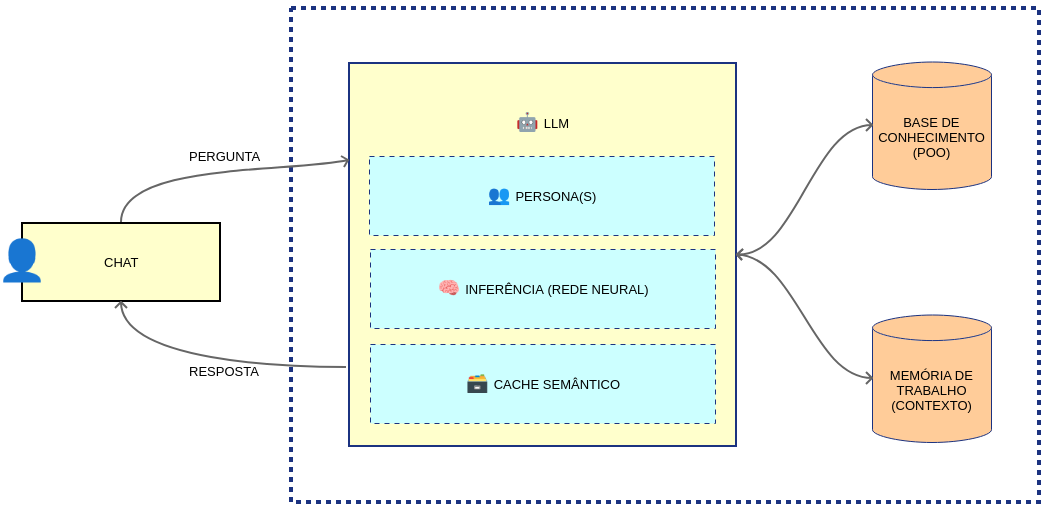
\includegraphics[width=1.0\textwidth]{capitulos/capitulo_1/arquitetura.png}
\caption{Arquitetura do ProgBot}
\label{fig:arquitetura-progbot}
\end{figure}

\section{Ferramentas MCP}

Quando uma aplicação com LLM se conecta a ferramentas por meio do MCP, o protocolo oferece uma interface padronizada para descobrir e invocar capacidades externas e incorporar os resultados ao fluxo de interação \cite{mcp2026architecture}. Assim, o sistema pode complementar a geração de texto com ações executadas por serviços especializados. No ProgBot, isso permite combinar as respostas do modelo com verificações de linguagem de programação e sintaxe, oferecendo retorno mais contextualizado e prático ao usuário.

O ProgBot disponibiliza duas ferramentas: \path{detectar_linguagem}, que identifica a linguagem de programação utilizada em um trecho de código, evitando que o usuário precise informá-la manualmente; e \path{verificar_sintaxe}, que confere se o código segue as regras sintáticas da linguagem indicada e aponta quando há erros. Em conjunto, elas facilitam a análise inicial do código e ajudam o usuário a localizar problemas de sintaxe.

\section{Desenvolvimento e Avaliação}

O ProgBot foi desenvolvido em Python, integrando bibliotecas com funções complementares. A \textit{sentence-transformers} converte perguntas e trechos da base de conhecimento em \textit{embeddings}, que possibilitam comparar a similaridade entre a consulta e os conteúdos. O \textit{chromadb} armazena vetores de representação numérica dos \textit{embeddings}. A biblioteca, \textit{google-genai}, permite enviar instruções e contexto à API do Gemini e receber a resposta gerada. O \texttt{FastMCP} é usado para disponibilizar ferramentas e recursos por meio do protocolo MCP. Desse modo, conteúdos recuperados podem ser fornecidos ao modelo como contexto adicional para processamento de código-fonte. 

O resultado da união desses recursos pode ser visto na Figura \ref{fig:funcionamento-progbot}. É possível visualizar a interação do usuário com o ProgBot e também a possibilidade de uso das ferramentas MCP.

\begin{figure}[htbp]
\centering
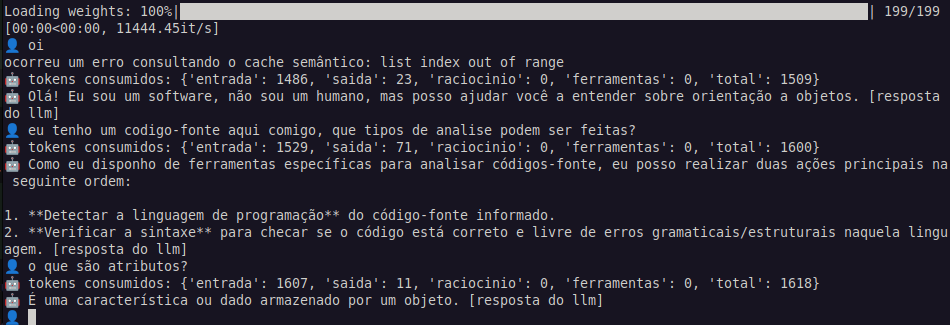
\includegraphics[width=1.0\textwidth]{capitulos/capitulo_1/funcionamento.png}
\caption{Funcionamento do ProgBot}
\label{fig:funcionamento-progbot}
\end{figure}

Para testar a qualidade das respostas, aplica-se a técnica \textit{LLM-as-a-Judge}. Para cada pergunta de avaliação, um julgador analisa a pergunta e a resposta do ProgBot. Respostas que não são consideradas adequadas podem ser usadas para identificar ajustes necessários nos \textit{prompts} ou na escolha dos LLMs utilizados para realizar as inferências sobre as perguntas do usuários. O resultado do julgamento pode ser visto na Figura \ref{fig:julgamento-progbot}.

\begin{figure}[htbp]
\centering
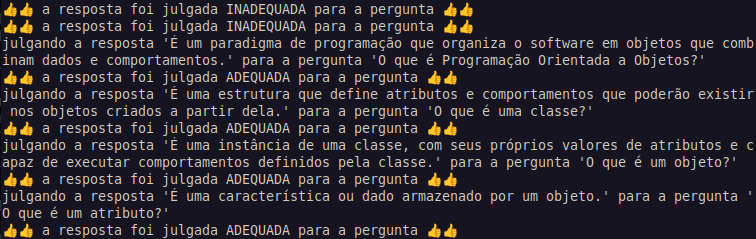
\includegraphics[width=1.0\textwidth]{capitulos/capitulo_1/julgamento.png}
\caption{Julgamento do ProgBot}
\label{fig:julgamento-progbot}
\end{figure}

\section{Reproducibilidade e Reuso}

O código-fonte do ProgBot pode ser consultado e (re)usado livremente através do link de acesso ao \href{https://zenodo.org/records/23445337?preview_file=progbot.zip}{repositório do projeto}. Também se encontra disponibilizado um vídeo demonstrativo \href{https://zenodo.org/records/23428906/preview/progbot.mp4}{neste link}. 
\chapter{PlantaBot - Um Sistema Especialista para Supervisão e Manutenção de Planta Industrial}

\begin{flushright}
Sid Gubert
\end{flushright}

PlantaBot é um Assistente Virtual Especialista em Supervisão e Manutenção Preditiva de Planta Industrial, integrado ao ecossistema supervisório \textit{PlantaView}. O seu objetivo é auxiliar operadores de sala de controle, técnicos e engenheiros de manutenção no diagnóstico em tempo real de anomalias operacionais, na interpretação de grandezas físicas (temperatura, pressão, vazão e vibração mecânica) e na priorização de ordens de serviço.

Nos sistemas supervisórios industriais do tipo SCADA (\textit{Supervisory Control and Data Acquisition}), o volume contínuo de telemetria e a ocorrência simultânea de eventos de alarme exigem respostas rápidas e precisas para evitar paradas não programadas ou danos severos a ativos críticos \cite{mobley2002introduction}. A integração de Sistemas Especialistas baseados em Grandes Modelos de Linguagem (LLMs) com bases de conhecimento normativas, como os critérios de severidade de vibração da norma ISO 10816 \cite{iso10816} e protocolos de bloqueio de segurança LOTO (\textit{Lockout/Tagout}), permite transformar dados brutos de sensores em recomendações prescritivas acionáveis \cite{yang2025comprehensive,garridomerchan2026gofai}.

O desenvolvimento do PlantaBot uniu a inferência local via modelos de linguagem executados no servidor \textit{Ollama} com a consulta determinística a ferramentas industriais via protocolo MCP (\textit{Model Context Protocol}). A solução utiliza \textit{prompts} estruturados para configurar uma persona especialista em engenharia de manutenção industrial, disponibilizando uma interface conversacional (\textit{chat}) capaz de correlacionar histórico de sensores, alarmes ativos e ordens de manutenção.

As seções seguintes descrevem a arquitetura do sistema, o conjunto de ferramentas MCP desenvolvidas para inspeção da planta, o fluxo de implementação e validação automatizada e as instruções para reprodução e reuso da solução.

\section{Arquitetura do PlantaBot}

A Figura \ref{fig:arquitetura-plantabot} apresenta a arquitetura de interfaces e componentes do PlantaBot. O operador interage com o núcleo do Sistema Especialista por meio de uma interface de \textit{chat}. Ao receber uma consulta, o sistema verifica inicialmente a aderência ao domínio industrial (\textit{guardrails} de escopo) e consulta a memória de trabalho. O núcleo de inferência é composto por um LLM local servido via \textit{Ollama} (\texttt{qwen2.5:1.5b} ou \texttt{qwen3:4b}), parametrizado por um \textit{prompt} de sistema que incorpora as regras operacionais e os procedimentos de manutenção da base de conhecimento (\path{conhecimento/planta.json}), abstendo-se de responder a questões alheias à operação da planta industrial. A memória de trabalho combina dois mecanismos complementares: (i) um cache semântico vetorial, capaz de recuperar instantaneamente respostas para perguntas semanticamente equivalentes a consultas já processadas (distância de cosseno $\le 0{,}20$), e (ii) o histórico conversacional mantido na sessão de inferência junto ao motor LLM.

\begin{figure}[htbp]
\centering
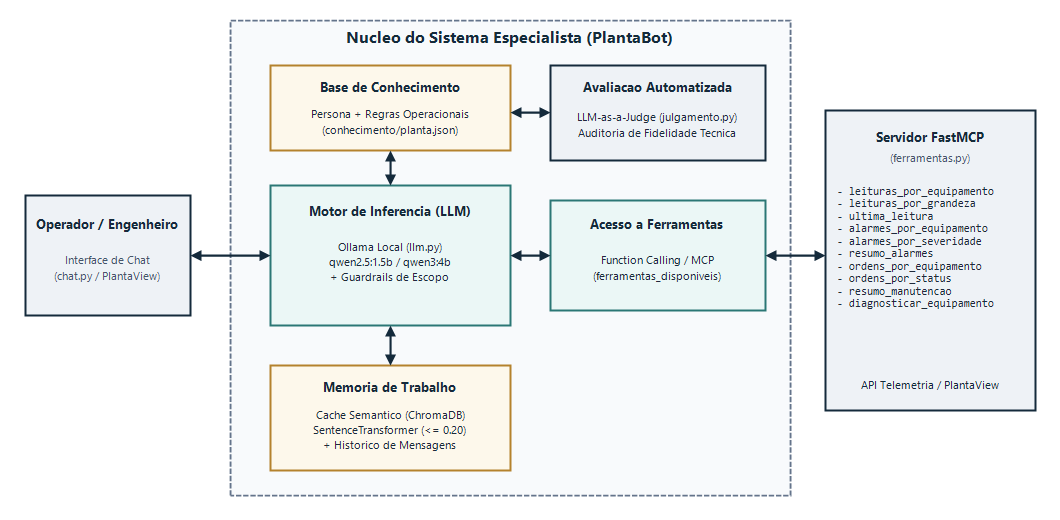
\includegraphics[width=1.0\textwidth]{capitulos/capitulo_2/arquitetura.png}
\caption{Arquitetura do PlantaBot}
\label{fig:arquitetura-plantabot}
\end{figure}

\section{Ferramentas MCP}

Por meio do protocolo MCP \cite{mcp2026architecture}, o PlantaBot conecta o motor de inferência diretamente aos dados operacionais dos ativos monitorados na planta industrial (Bomba Centrífuga Principal \texttt{EQ-001}, Compressor de Ar Industrial \texttt{EQ-002}, Caldeira de Vapor \texttt{EQ-003}, Torre de Resfriamento \texttt{EQ-004} e Motor Elétrico Trifásico \texttt{EQ-005}). Dessa forma, sempre que o operador questiona o estado atual de um equipamento, o modelo invoca automaticamente a ferramenta apropriada (\textit{function calling}) e fundamenta seu parecer técnico nos indicadores reais da planta.

O servidor MCP do PlantaBot disponibiliza dez ferramentas organizadas em quatro categorias operacionais: (i) monitoramento de sensores: \path{leituras_por_equipamento}, \path{leituras_por_grandeza} e \path{ultima_leitura}, que retornam séries históricas, estatísticas (mínimo, máximo, média e tendência por hora) e limites operacionais de cada sensor; (ii) gestão de alarmes: \path{alarmes_por_equipamento}, \path{alarmes_por_severidade} e \path{resumo_alarmes}, que filtram eventos ativos ou reconhecidos segundo a criticidade (\texttt{CRITICO}, \texttt{ALTO}, \texttt{MEDIO} e \texttt{BAIXO}); (iii) controle de manutenção: \path{ordens_por_equipamento}, \path{ordens_por_status} e \path{resumo_manutencao}, que consultam ordens de serviço preventivas e corretivas; e (iv) diagnóstico integrado: \path{diagnosticar_equipamento}, que consolida leituras em anomalia, tendência térmica/mecânica, alarmes ativos e ordens pendentes para emitir um laudo completo do ativo.

\section{Desenvolvimento e Avaliação}

O PlantaBot foi implementado em linguagem Python, integrando bibliotecas voltadas à recuperação semântica, inferência em LLMs e exposição de serviços MCP. A biblioteca \textit{sentence-transformers} (\texttt{paraphrase-multilingual-MiniLM-L12-v2}) converte tanto as regras da base de conhecimento quanto as dúvidas dos operadores em vetores densos (\textit{embeddings}), os quais são persistidos e consultados na base vetorial \textit{chromadb}. A comunicação com o motor de inferência local no \textit{Ollama} é realizada pelo módulo \path{llm.py}, que gerencia o envio de contexto, a remoção automática de blocos intermediários de raciocínio (\textit{thinking tags}) e o ciclo de invocação das ferramentas registradas via \texttt{FastMCP} (\path{ferramentas.py}).

A Figura \ref{fig:funcionamento-plantabot} ilustra o funcionamento do PlantaBot em execução. Observa-se tanto o acionamento automático da ferramenta MCP \path{diagnosticar_equipamento} para inspecionar a Bomba Centrífuga Principal (\texttt{EQ-001}) quanto a recuperação imediata pelo cache semântico em consultas normativas sobre faixas operacionais.

\begin{figure}[htbp]
\centering
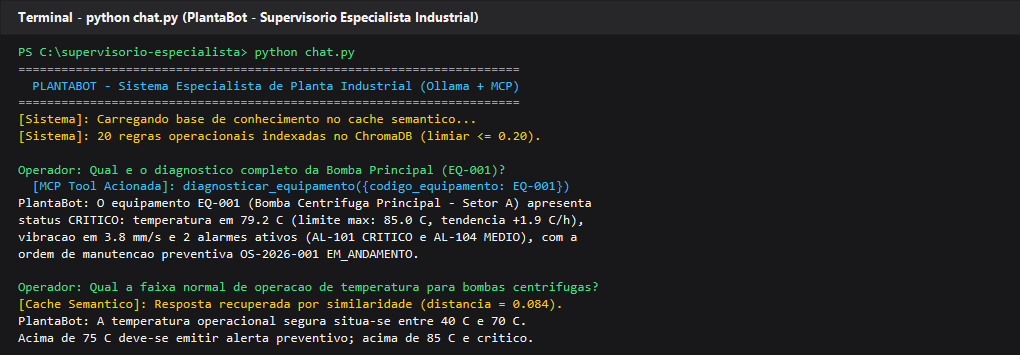
\includegraphics[width=1.0\textwidth]{capitulos/capitulo_2/funcionamento.png}
\caption{Funcionamento do PlantaBot}
\label{fig:funcionamento-plantabot}
\end{figure}

Para aferir de forma sistemática a qualidade e a fidelidade técnica das respostas geradas pelo especialista, aplicou-se a técnica \textit{LLM-as-a-Judge} \cite{azevedo2026julgamento} por meio do script \path{julgamento.py}. Nessa etapa, o modelo especialista (\texttt{qwen2.5:1.5b}) responde às questões de referência da planta industrial sem auxílio do cache pré-carregado, enquanto um modelo julgador independente de maior capacidade (\texttt{qwen3:4b}) avalia cada resposta gerada em comparação ao gabarito de engenharia de manutenção, classificando-a como adequada ou inadequada com justificativa técnica. O resultado da avaliação automatizada é apresentado na Figura \ref{fig:julgamento-plantabot}.

\begin{figure}[htbp]
\centering
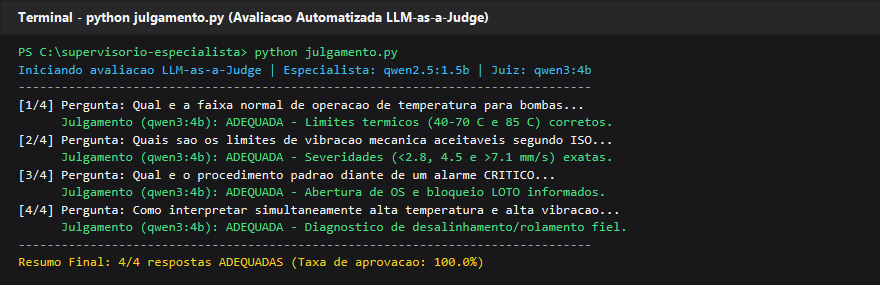
\includegraphics[width=1.0\textwidth]{capitulos/capitulo_2/julgamento.png}
\caption{Julgamento do PlantaBot}
\label{fig:julgamento-plantabot}
\end{figure}

\section{Reproducibilidade e Reuso}

O código-fonte completo do PlantaBot (Supervisório Especialista), incluindo a base de conhecimento industrial, o servidor de ferramentas MCP, os testes automatizados e o avaliador \textit{LLM-as-a-Judge}, pode ser consultado e (re)usado livremente através do link de acesso ao \href{https://zenodo.org/records/supervisorio-especialista?preview_file=supervisorio-especialista.zip}{repositório do projeto} (também disponível em \url{https://github.com/sidgubert/supervisorio-especialista}). Também se encontra disponibilizado um vídeo demonstrativo \href{https://zenodo.org/records/supervisorio-especialista/preview/plantabot.mp4}{neste link}.

\normalsize
\backmatter
\nocite{*}
\printbibliography[heading=bibintoc,title={Referências}]
\end{document}
